\chapter{Systèmes linéaires}

\noindent Voyons ici une première application importante des objets mathématiques introduits dans la section précédente, les matrices : les \textit{systèmes d'équations linéaires}. Tout d'abord qu'est ce qu'une équation linéaire ? Il s'agit d'une égalité faisant intervenir une somme d'inconnues chacune multipliées par un coefficient réel. 

\section{Définition et exemples, intuition géométrique}
\begin{boxdef}
\noindent Une \textit{équation linéaire} est une équation de la forme : 
$$a_1 x_1 + ... + a_n x_n = b$$
avec $\{a_i \}_{i \in \Iintv{1,n}} \subseteq \mathbb{R}$ et $b\in \mathbb{R}$. Nous appelons $n$ le nombre \textit{d'inconnues}. Un \textit{système} d'équations linéaires est caractérisé par un ensemble \textit{fini} d'équations linéaires.
\end{boxdef}
Plus précisément nous pouvons donc représenter une équation linéaire sous la forme :
$$a_1 x_1 + ... + a_n x_n = b
$$
où les $a_i \in \R$ et $b \in \R$ sont connus, puis écrire un système linéaire :
$$\begin{cases} a_{1,1}x_1 + a_{1,2}x_2 + a_{1,3}x_3 + ... + a_{1, n}x_n = b_1 \\ a_{2,1}x_1 + a_{2,2}x_2 + a_{2,3}x_3 + ... + a_{2, n}x_n =b_2 \\ \vdots \\ a_{p,1}x_1 + a_{p,2}x_2 + a_{p,3}x_3 + ... + a_{p, n}x_n = b_p \end{cases}$$

\, \\
Avant de continuer, un peu de vocabulaire:
\begin{boxdef}
Un système linéaire à $n$ inconnues et $p$ équations est dit \textit{homogène} si $b_i = 0$ $\forall i \in \Iintv{1, p}$.
\end{boxdef}

\noindent Le plus souvent, la donnée intéressante d'un système d'équations linéaires est son ensemble de solutions, c'est à dire le tuple des $(y_1, y_2, \ldots, y_n)\in \mathbb{R}^n$ tels que pour chaque équation du système, en injectant ces valeurs dans les $x_n$ on obtienne bien $b_i$. Notons pour l'instant cet ensemble de solutions $S(\{a_{i,j}\},b)$. Concentrons-nous sur quelques équations simples pour visualiser géométriquement à quoi ressemblent ces ensembles de solutions.\\

\noindent Tout d'abord remarquons que pour un système d'équations à $n$ variables, $S(\{a_{i,j}\}, b)$ est un sous ensemble de $\mathbb{R}^n$ puisqu'il est constitué de $n$-uplets de réels. Commençons donc avec des sous ensembles de $\mathbb{R}^2$, à savoir des sous ensembles du plan. 
$$ 2x_1 - x_2 = 0 $$
\noindent Ceci est l'équation d'une droite. Ici nous commençons par remarquer qu'il s'agit d'un système à une équation et deux variables, nous avons, selon la notation précédente $a_{1,1} =2 $, $a_{1,2} = -1$ et  $b_1 = 0$. Remarquons qu'il s'agit d'un système homogène. Nous résolvons en passant simplement le $x_2$ de l'autre coté on obtient :
$$2x_1 = x_2$$
Il s'agit donc de l'ensemble des $(x_1, x_2) \in \mathbb{R}^2$ tels que $2x_1 = x_2$. Nous pourrons alors aussi dire qu'il s'agit, pour tout $x\in \mathbb{R}$ des $(x, 2x)$. Géométriquement à quoi correspond cet ensemble ? Remarquons que comme $x$ est réel il s'agit bien de l'ensemble des $\left\{x\begin{bmatrix}1 \\ 2 \end{bmatrix} \ | \ x \in \R\right\}$. Visuellement le vecteur $\begin{bmatrix}1 \\ 2 \end{bmatrix}$ est représenté ci dessous. L'ensemble des vecteurs obtenus en lui multipliant un réel $x$ sont représentés sur la figure de droite:
\begin{center}
\begin{tikzpicture}

  \draw[thin,gray!40] (-3,-3) grid (3,3);
  \draw[<->] (-3,0)--(3,0) node[right]{$x$};
  \draw[<->] (0,-3)--(0,3) node[above]{$y$};
  \draw[line width=2pt,blue,-stealth](0,0)--(1,2) node[anchor=south west]{$\begin{bmatrix}1 \\ 2 \end{bmatrix}$};
\end{tikzpicture}
\hspace{2CM}
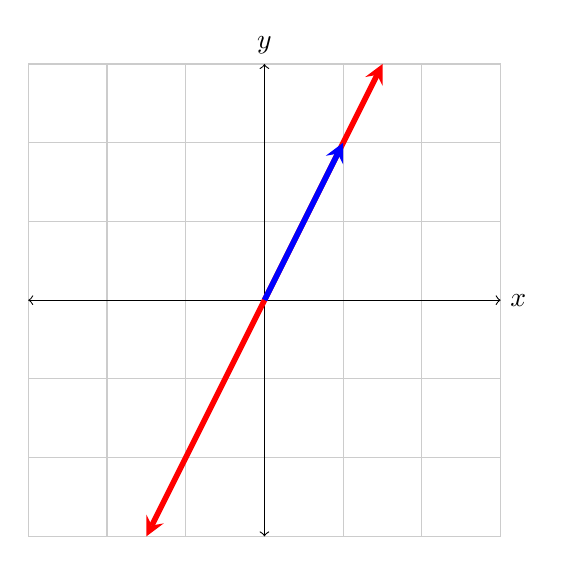
\begin{tikzpicture}
  \draw[thin,gray!40] (-3,-3) grid (3,3);
  \draw[<->] (-3,0)--(3,0) node[right]{$x$};
  \draw[<->] (0,-3)--(0,3) node[above]{$y$};
    \draw[line width=2pt,red,-stealth](0,0)--(1.5,3) node[anchor=south west]{};
  \draw[line width=2pt,blue,-stealth](0,0)--(1,2) node[anchor=south west]{};
  \draw[line width=2pt,red,-stealth](0,0)--(-1.5,-3) node[anchor=south west]{};

\end{tikzpicture}
\end{center}
Il s'agit donc d'une droite dirigée par le vecteur $\begin{bmatrix}1 \\ 2 \end{bmatrix}$. Prenons désormais un exemple avec un système à trois inconnues et deux équations :

$$ \begin{cases}3x_1 + 2x_2 + x_3 = 2\\x_1 + 2x_2 + x_3 = 2 \end{cases}$$
%yeet
%who is the author of this yeet?
Comment procéder à la résolution ? Soustrayons la deuxième équation à la première pour obtenir :

$$ \begin{cases}2x_1  = 0\\ x_1 + 2x_2 + x_3 = 2 \end{cases}$$

\noindent Et donc conclure déjà que les points de notre ensemble de solution seront de la forme $(0, x_2, x_3)\in \mathbb{R}^3$ en divisant des deux cotés de $ 2x_1  = 0$ par $2$. Remplaçons donc $x_1$ par $0$ dans la seconde équation pour obtenir :
$$ 2x_2 + x_3 = 2 $$
\noindent Il s'agit encore une fois de l'équation d'une droite, ici de la droite dirigée par $$\begin{bmatrix}0 \\ 1 \\ -2 \end{bmatrix}$$ mais décalée de $2$ au niveau de l'origine :
\\
\begin{tikzpicture}

\pgfplotsset{
colormap={whitered}{color(0cm)=(white); color(1cm)=(orange!75!red)}
}

\begin{axis}[  colormap name=whitered,   view={45}{65},     width=10cm]
\addplot3[variable=t, mesh, draw=red!50, domain=-2:2] (0,{t + 2},{-2*t});
\end{axis}
\end{tikzpicture}
\hspace{1CM}
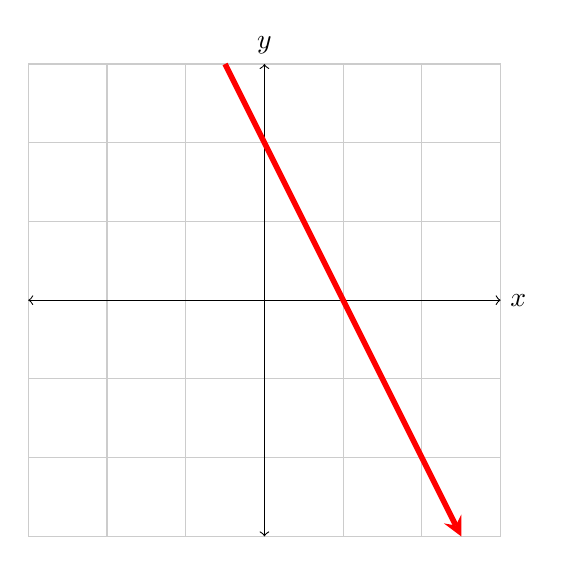
\begin{tikzpicture}
  \draw[thin,gray!40] (-3,-3) grid (3,3);
  \draw[<->] (-3,0)--(3,0) node[right]{$x$};
  \draw[<->] (0,-3)--(0,3) node[above]{$y$};
    \draw[line width=2pt,red,-stealth](-0.5,3)--(2.5,-3) node[anchor=south west]{};

\end{tikzpicture}
A droite est une coupe selon l'axe des $x_1 = 0$. 
\section{L'équation $Ax = b$}
\noindent Reprenons une équation connue et cherchons les informations capitales à son sujet : 
$$ \begin{cases}5x_1 + x_3 = \sqrt{2}\\x_1 + 3x_2 +4x_3 = 3\end{cases} $$
\noindent Quelles sont les informations minimales dont on a besoin pour reconstituer une telle équation ? Les variables peuvent être ordonnées de sorte à toujours apparaître dans le même ordre. Nous pourrions aussi omettre le signe "$=$" en sachant que le dernier coefficient est celui correspondant à $b_i$. Enfin nous pourrions encore omettre le nom des variables et ne conserver que les coefficients puisque l'ordre des coefficients détermine la variable qu'ils multiplient. Et que faire si l'une des variables n'est pas présente ? Il s'agit bien de la multiplication par $0$ dans ce cas. En résumé nous obtenons :
$$ 5 \quad 0 \quad 1 \quad \sqrt{2}$$
$$ 1 \quad 3 \quad 4 \quad 3 $$
Nous pouvons réécrire cela de manière plus élégante sous la forme :
$$ 
\left[
\begin{array}{@{}ccc|c@{}}
5 & 0 & 1 & \sqrt{2} \\
1 & 3 & 4 & 3 \\
\end{array}
\right]
$$
\noindent Voici la forme \textit{matricielle augmentée} d'un système linéaire. Cette forme est équivalente à la donnée de l'équation suivante dite \textit{équation matricielle} $Ax = b$ :
$$\underbrace{\begin{bmatrix}
5 & 0 & 1 \\
1 & 3 & 4 
\end{bmatrix}}_{A}\underbrace{\begin{bmatrix}
x_1 \\ x_2 \\ x_3
\end{bmatrix}}_{x} = \underbrace{\begin{bmatrix}
\sqrt{2} \\ 2
\end{bmatrix}}_{b}
$$
Dans cette notation, $A$ est la \textit{matrice des coefficients}, et la \textit{matrice augmentée} de l'équation matricielle est ainsi $\begin{bmatrix}
A & | & b
\end{bmatrix}$.

Cela aboutit à cette définition générale:
\begin{boxdef}
Étant donné un système linéaire
$$\begin{cases} a_{1,1}x_1 + a_{1,2}x_2 + a_{1,3}x_3 + ... + a_{1, n}x_n = b_1 \\ a_{2,1}x_1 + a_{2,2}x_2 + a_{2,3}x_3 + ... + a_{2, n}x_n =b_2 \\ \vdots \\ a_{p,1}x_1 + a_{p,2}x_2 + a_{p,3}x_3 + ... + a_{p, n}x_n = b_p \end{cases}$$
On note $b \in \R^p$ le vecteur formé par les $b_i$ et on défini la \textit{matrice des coefficients} comme étant
$$A = \begin{bmatrix}
a_{1,1} & a_{1,2} & \cdots & a_{1,n} \\
a_{2,1} & a_{2,2} & \cdots & a_{2,n} \\
\vdots & \vdots & \ddots & \vdots \\
a_{p,1} & a_{p,2} & \cdots & a_{p,n} \\
\end{bmatrix}$$
La \textit{matrice augmentée} du système est donc $\begin{bmatrix}
A & | & b
\end{bmatrix}$.
\end{boxdef}

\section{Réduction et échelonnage}
\noindent Soit le système linéaire :
$$\begin{cases}
3x_1 + 2x_2 + x_3 = 2\\
x_1 + 2x_2 + x_3 = 2
\end{cases}
$$
La matrice augmentée associée est alors :
$$ 
\left[
\begin{array}{@{}ccc|c@{}}
3 & 2 & 1 & 2 \\
1 & 2 & 1 & 2 \\
\end{array}
\right]
$$
Résolvons ce système sous les deux écritures i.e système et matrice augmentée simultanément. Soustrayons donc chaque coefficient de la seconde ligne au coefficient correspondant de la ligne supérieure pour obtenir :
$$ 
\left[
\begin{array}{@{}ccc|c@{}}
3 \color{red} - 1 & 2 \color{red} -2 & 1  \color{red} - 1 & 2 \color{red} - 2 \\
1 & 2 & 1 & 2 \\
\end{array}
\right] 
\iff 
\begin{cases}
(3\textcolor{red}{-1})x_1 + (2\textcolor{red}{-2})x_2 + (1\textcolor{red}{-1})x_3 = 2\textcolor{red}{-2}\\
x_1 + 2x_2 + x_3 = 2
\end{cases}
$$

$$ 
\left[
\begin{array}{@{}ccc|c@{}}
2 & 0 & 0 & 0 \\
1 & 2 & 1 & 2 \\
\end{array}
\right]
\iff
\begin{cases}
2x_1 = 0\\
x_1 + 2x_2 + x_3 = 2
\end{cases}
$$
Nous multiplions ensuite les coefficients de la première ligne par $\color{blue}\frac{1}{2}$ :
$$ 
\left[
\begin{array}{@{}ccc|c@{}}
2 \color{blue}\times\frac{1}{2}  & 0 & 0 & 0 \\
1 & 2 & 1 & 2 \\
\end{array}
\right]
\iff
\begin{cases}
2\textcolor{blue}{\times \frac{1}{2}}x_1 = 0\\
x_1 + 2x_2 + x_3 = 2
\end{cases}
$$
$$ 
\left[
\begin{array}{@{}ccc|c@{}}
1 & 0 & 0 & 0 \\
1 & 2 & 1 & 2 \\
\end{array}
\right]
\iff
\begin{cases}
x_1 = 0 \\
x_1 + 2x_2 + x_3 = 2
\end{cases}
$$
Et nous concluons alors que le premier coefficient est nul.\\
Continuons en soustrayant la première ligne à la seconde :
$$ 
\left[
\begin{array}{@{}ccc|c@{}}
1 & 0 & 0 & 0 \\
1\color{red} - 1 & 2\color{red} - 0 & 1\color{red} - 0 & 2\color{red} - 0 \\
\end{array}
\right]
\iff 
\begin{cases}
x_1 = 0 \\
(1\textcolor{red}{-1})x_1 + (2\textcolor{red}{-0})x_2 + (1\textcolor{red}{-0})x_3 = 2\textcolor{red}{-0}
\end{cases}
$$
$$ 
\left[
\begin{array}{@{}ccc|c@{}}
1 & 0 & 0 & 0 \\
0 & 2 & 1 & 2 \\
\end{array}
\right]
\iff
\begin{cases}
x_1 = 0 \\
2x_2 + x_3 = 2
\end{cases}
$$
Nous pouvons peut être aller un peu plus loin en divisant la deuxième ligne par 2, ce qui donne :
$$
\left[
\begin{array}{@{}ccc|c@{}}
1 & 0 & 0 & 0 \\
0 & 1 & \frac{1}{2} & 1 \\
\end{array}
\right]
\iff
\begin{cases}
x_1 = 0 \\
x_2 + \frac{1}{2}x_3 = 1
\end{cases}
$$
Formalisons les opérations que nous pouvons utiliser pour résoudre un système linéaire sous sa forme matricielle, qui sont en fait les mêmes que celle sous sa forme de système d'équations linéaires : 
\begin{itemize}
    \item \textit{La multiplication par un réel non nul} d'une ligne complète (ne pas oublier le $b_i$).
    \item \textit{Additionner deux lignes} (la soustraction correspond à multiplier la ligne par $-1$ puis l'additionner à l'autre et la multiplier à nouveau par $-1$).
    \item \textit{Permuter deux lignes}, la permutation de deux équations dans un système étant sans conséquence.
\end{itemize}
\textbf{Notons d'abord que ces trois opérations sont réversibles. C'est ce qui fait que l'ensemble des solutions n'est pas changé par ces 3 opérations.}\\

\noindent Remarquons aussi que nous pouvons toujours procéder comme dans la soustraction et multiplier la $i$ème ligne par un réel $\lambda \in \mathbb{R}^*$, l'additionner à la $j$-ème ligne et multiplier à nouveau la $i$ème ligne par $\frac{1}{\lambda}$. Nous en concluons une règle composite très pratique : 
\begin{itemize}
    \item \textit{La multiplication puis l'addition} d'une ligne vers une autre sans modifier sa propre valeur.
\end{itemize}
Il s'agit désormais de trouver un algorithme qui pourrait toujours mener vers la forme la plus réduite possible d'une équation, commençons par trouver les critères qu'une telle forme doit posséder. Tout d'abord on remarque que les lignes de la forme 
$$ 
\left[
\begin{array}{@{}ccccc|c@{}}
0 & \ldots & \lambda & \ldots & 0 & \sigma \\
\end{array}
\right]
\iff
0x_1 + \cdots + \lambda x_i + 0x_{i+1} + \cdots + 0x_n = \sigma
$$
pour tout $\lambda \in \R^*, \sigma \in \mathbb{R}$ sont très pratiques puisqu'elles déterminent la valeur de la variable dont le coefficient n'est pas nul de manière unique : $x_i = \frac{\sigma}{\lambda}$. Il s'agirait donc d'obtenir une matrice qui maximise le nombre de ligne de cette forme.\\

\noindent Remarquons que si nous disposons d'une ligne de la forme :
$$ 
\left[
\begin{array}{@{}ccccc|c@{}}
0 & \ldots & \lambda_1 & \ldots & \lambda_n & \sigma \\
\end{array}
\right]
$$
\noindent Alors pour annuler les derniers coefficients (sur la droite) il faut déjà avoir une ligne qui contienne au plus autant de coefficients non nuls à droite sans quoi lors de l'addition des lignes nous créerons des termes non nuls là où nous avions déjà des termes nuls :
$$ 
\left[
\begin{array}{@{}ccccc|c@{}}
0 \color{green} -0  & 0\color{green} -0 & \lambda_1 \color{green} -\alpha_1 & \lambda_2 \color{green} -\alpha_2 & \lambda_3\color{green} -\alpha_3 & \sigma_1\color{green} -\sigma_2 \\
0 & 0  & \alpha_1 & \alpha_2 & \alpha_3 & \sigma_2 \\
\end{array}
\right]
$$
Ci-dessus une soustraction n'ajoutant pas de termes, et ci après une soustraction ajoutant des termes non nuls.
$$ 
\left[
\begin{array}{@{}ccccc|c@{}}
0 \color{green} -0  & 0\color{red} -\alpha_0 & \lambda_1 \color{green} -\alpha_1 & \lambda_2 \color{green} -\alpha_2 & \lambda_3\color{green} -\alpha_3 & \sigma_1\color{green} -\sigma_2 \\
0 & \alpha_0  & \alpha_1 & \alpha_2 & \alpha_3 & \sigma_2 \\
\end{array}
\right]
$$
Nous constatons donc que pour arriver à obtenir une forme matricielle contenant le plus de lignes avec un seul terme non nul il conviendrait premièrement d'en trouver une dont les lignes auraient un \textit{nombre de termes non nul à droite décroissant}, c'est-à-dire telle que : si $A \in \R^{p \cross n}$, alors pour tout $i \in \Iintv{1,p}$, si la colonne $k\in \Iintv{1,n}$ est la première colonne de la $i$ème ligne dont le coefficient est non nul, alors le rang de la première colonne de la $i+1$ème ligne dont le coefficient est non nul est strictement supérieur à $k$. \\

Dans la matrice suivante, $*$ désigne un coefficient arbitraire, et les $\Delta_i$ désignent des coefficients \textit{non nuls} arbitraires.
$$\begin{bmatrix}
0 & \cdots & 0 & \Delta_1 & * & \cdots & * & * & *\\
0 &\cdots & 0 & 0 & \cdots & \Delta_2 & * &\cdots & *\\
\vdots &&&&&&&&\vdots \\
0 & &&\cdots&&\cdots&&& *
\end{bmatrix}
$$
\begin{boxdef}
La forme ci-dessus est appelée la forme \textit{échelonnée} d'une matrice. Les premiers termes non nuls sur une ligne sont appelés \textit{pivots}.
\end{boxdef}
En d'autres termes, les coefficients non nuls font une sorte d'escalier plus ou moins régulier. Des exemples de matrices sous forme échelonnée, avec, en bleu, les pivots :
$$
\begin{bmatrix}
\color{blue}5 & 0 & 3 & 3 \\
0 & 0 & \color{blue}2 & 1 \\
0 & 0 & 0 & 0
\end{bmatrix},
\begin{bmatrix}
0 & 0 \\
0 & 0
\end{bmatrix},
\begin{bmatrix}
\color{blue}1 & 0\\
0 & \color{blue}1\\
0 & 0
\end{bmatrix},
\begin{bmatrix}
0 & 0 & 0 & 0 & 0 \\
0 & 0 & 0 & \color{blue}5 & 4
\end{bmatrix}
$$
Des exemples de matrices \textit{pas} sous forme échelonnée :
$$
\begin{bmatrix}
0 & 2 & 3 \\
1 & 5 & 6\\
0 & 9 & 1
\end{bmatrix},
\begin{bmatrix}
0 & 0 & 7 \\
0 & 4 & 0\\
0 & 0 & 0\\
0 & 0 & 0
\end{bmatrix}
$$
La première n'est pas échelonnée car le coefficient $1$ est en colonne $1$ de la ligne 2, soit avant le premier coefficient non nul de la ligne au-dessus, qui est $2$. Idem : le $4$ dans la seconde matrice est situé à la deuxième colonne alors que la première ligne compte le coefficient non nul 7 à la troisième colonne.\\

\noindent Ensuite, étant donnée une forme échelonnée, il est encore possible de la réduire. Nous pouvons faire en sorte que tous les pivots valent $1$ et que tous les coefficients sur la même colonne au-dessus de chaque pivot deviennent nuls, et ce \textit{en divisant la ligne du pivot} par le pivot lui-même (non nul par définition), puis en soustrayant la ligne du pivot aux lignes du dessus. Ainsi, il faudra commencer par la ligne du-dessous.\\
\begin{boxdef}
Nous appelons cette forme celle de matrice \textit{échelonnée réduite}.\\
\end{boxdef}
Des exemples rendront ce texte cryptique  plus compréhensible :
\begin{align*}
\begin{bmatrix}
\color{blue}5 & 0 & 3 & 3\\
0 & 0 & \color{blue}2 & 1\\
0 & 0 & 0 & 0
\end{bmatrix} \overset{L_2 \to  \frac{1}{2}L_2}{\sim} 
&\begin{bmatrix}
\color{blue}5 & 0 & 3 & 3\\
0 & 0 & \color{blue}1 & \frac{1}{2}\\
0 & 0 & 0 & 0
\end{bmatrix}\\
\overset{L_1 \to L_1 - 3L_2}{\sim}
&\begin{bmatrix}
\color{blue}5 & 0 & 0 & \frac{3}{2}\\
0 & 0 & \color{blue}1 & \frac{1}{2}\\
0 & 0 & 0 & 0
\end{bmatrix}\\
\overset{L_1 \to \frac{1}{5}L_1}{\sim}
&\begin{bmatrix}
\color{blue}1 & 0 & 0 & \frac{3}{10}\\
0 & 0 & \color{blue}1 & \frac{1}{2}\\
0 & 0 & 0 & 0
\end{bmatrix}
\end{align*}
Puis, $\begin{bmatrix}
0 &0\\
0 & 0
\end{bmatrix}$ est déja échelonnée réduite. Idem, la matrice $\begin{bmatrix}
1 & 0\\
0 & 1\\
0 & 0
\end{bmatrix}$ l'est déjà aussi. Enfin :
\begin{align*}
\begin{bmatrix}
0 & 0 & 0 & 0 & 0 \\
0 & 0 & 0 & \color{blue}5 & 4
\end{bmatrix}
\overset{L_2 \to \frac{1}{5}L_2}{\sim}
\begin{bmatrix}
0 & 0 & 0 & 0 & 0 \\
0 & 0 & 0 & \color{blue}1 & \frac{4}{5}
\end{bmatrix}
\end{align*}
Nous verrons dans la prochaine section comment exploiter cette forme échelonnée réduite afin d'expliciter l'ensemble des solutions d'un système linéaire.\\

\noindent Il serait désormais utile de trouver un algorithme amenant à une forme échelonnée, puisque nous savons passer d'une forme échelonnée à une forme réduite désormais. La méthode présentée ci-après est celle du \textit{pivot de Gauss}.\\

\noindent Nous commencerons par un exemple. Calculons la forme échelonnée réduite de la matrice suivante :
$$\begin{bmatrix}
-1 & -2 & -1 & 3 \\
-2 & -3 &  0 & 3 \\
1  &  4 &  5 & -9
\end{bmatrix}
$$
\begin{mdframed}
Le but sera d'aller de la gauche vers la droite. Pour chaque colonne, nous sélectionnerons une ligne que nous trouverions "avantageuse" afin de simplifier les calculs, bien qu'en soi n'importe quelle ligne marcherait. Cette ligne sera placée au-dessus. Puis, nous ajoutons des multiples de cette ligne aux lignes en-dessous de manière à faire apparaître des 0 dans la colonne courante. Puis, nous bloquons la ligne du dessus et passons à la prochaine colonne jusqu'à avoir traité la colonne la plus à droite.
\end{mdframed}

\noindent Ici, en choisissant la 3ème ligne dans la matrice ci-dessus, i.e celle contenant un coefficient $1$ à sa gauche, nous pourrions simplement annuler le $-1$ et le $-2$ en ajoutant respectivement 1 et 2 fois la ligne 3. Au fur et à mesure, les pivots bloqués seront colorés en bleu.\\

\noindent Chaque chose en son temps. Mettons d'abord en évidence cette ligne 3 en la plaçant au-dessus :
$$\begin{bmatrix}
-1 & -2 & -1 & 3 \\
-2 & -3 &  0 & 3 \\
1  &  4 &  5 & -9
\end{bmatrix}
\overset{L_1 \leftrightarrow L_3}{\sim} 
\begin{bmatrix}
\color{blue}1  &  4 &  5 & -9\\
-2 & -3 &  0 & 3 \\
-1 & -2 & -1 & 3 
\end{bmatrix}
$$
Ensuite, faisons des $0$ apparaître sous ce premier futur pivot :
\begin{align*}
\begin{bmatrix}
\color{blue}1  &  4 &  5 & -9\\
-2 & -3 &  0 & 3 \\
-1 & -2 & -1 & 3 
\end{bmatrix}
\overset{L_2 \to L_2 + 2L_1}{\sim}
&\begin{bmatrix}
\color{blue}1  &  4 &  5 & -9\\
0 & 5 &  10 & -15 \\
-1 & -2 & -1 & 3 
\end{bmatrix}\\
\overset{L_3 \to L_3 + L_1}{\sim}
&\begin{bmatrix}
\color{blue}1  &  4 &  5 & -9\\
0 & 5 &  10 & -15 \\
0 & 2 & 4 & -6 
\end{bmatrix}
\end{align*}
Nous pourrions recommencer directement l'opération avec la seconde colonne comme le prescrit la méthode de Gauss, mais remarquons d'abord que les lignes 2 et 3 se ressemblent particulièrement et sont toutes deux multiples de $\begin{bmatrix}
0 & 1 & 2 & -3
\end{bmatrix}$, mettons cela en évidence :
\begin{align*}
\begin{bmatrix}
\color{blue}1  &  4 &  5 & -9\\
0 & 5 &  10 & -15 \\
0 & 2 & 4 & -6 
\end{bmatrix}
\overset{L_3 \to \frac{1}{2}L_3}{\sim}
&\begin{bmatrix}
\color{blue}1  &  4 &  5 & -9\\
0 & 5 &  10 & -15 \\
0 & 1 & 2 & -3 
\end{bmatrix}\\
\overset{L_2 \to \frac{1}{5}L_2}{\sim}
&\begin{bmatrix}
\color{blue}1  &  4 &  5 & -9\\
0 & 1 & 2 & -3 \\
0 & 1 & 2 & -3 
\end{bmatrix}
\end{align*}
Il ne reste plus qu'à \textbf{yeet} la 2ème ligne - c'est un terme technique signifiant soustraire la 3ème à la 2ème \, ;)
$$
\begin{bmatrix}
\color{blue}1  &  4 &  5 & -9\\
0 & 1 & 2 & -3 \\
0 & 1 & 2 & -3 
\end{bmatrix}
\overset{L_2 \to L_2 - L_3}{\sim}
\begin{bmatrix}
\color{blue}1  &  4 &  5 & -9\\
0 & 0 & 0 & 0 \\
0 & 1 & 2 & -3 
\end{bmatrix}
$$
Nous avons presque une forme échelonnée ! Il reste encore à permuter les deux dernières lignes :
$$
\begin{bmatrix}
\color{blue}1  &  4 &  5 & -9\\
0 & 0 & 0 & 0 \\
0 & 1 & 2 & -3 
\end{bmatrix}
\overset{L_2 \leftrightarrow L_3}{\sim}
\begin{bmatrix}
\color{blue}1  &  4 &  5 & -9\\
0 & \color{blue}1 & 2 & -3 \\
0 & 0 & 0 & 0
\end{bmatrix}
$$
Enfin, pour arriver à la forme échelonnée réduite, en faisant donc apparaître un 0 au-dessus du second (et dernier) pivot, il suffira de retrancher la ligne 2 à la première ligne 4 fois :
$$
\begin{bmatrix}
\color{blue}1  &  4 &  5 & -9\\
0 & \color{blue}1 & 2 & -3 \\
0 & 0 & 0 & 0
\end{bmatrix}
\overset{L_1 \to L_1 - 4L_2}{\sim}
\begin{bmatrix}
\color{blue}1  &  0 &  -3 & 3\\
0 & \color{blue}1 & 2 & -3 \\
0 & 0 & 0 & 0
\end{bmatrix}
$$

\noindent Encore un exemple, issu du Lay, le livre de cours, que nous recommandons d'ailleurs pour son cours très clair, ses exemples d'applications de méthodes calculatoires proprement expliquées, mais pas pour ses exercices plus théoriques pour lesquels il faudra privilégier les séries d'exercices. Ceci est l'exemple 3 de la section 1.2 : Méthode du pivot de Gauss et formes échelonnées, qui est expliqué différemment dans le livre, et nous vous invitons à comparer sa méthode à celle présentée ci-après. \\

\noindent Trouvons la forme échelonnée réduite de la matrice suivante :
$$
\begin{bmatrix}
 0 &  3 & -6 &  6 &  4 & -5\\
 3 & -7 &  8 & -5 &  8 &  9\\
 3 & -9 & 12 & -9 &  6 & 15
\end{bmatrix}
$$
Avant de commencer, la troisième ligne est simplifiable par 3.
$$
\begin{bmatrix}
 0 &  3 & -6 &  6 &  4 & -5\\
 3 & -7 &  8 & -5 &  8 &  9\\
 3 & -9 & 12 & -9 &  6 & 15
\end{bmatrix}
\overset{L_3 \to \frac{1}{3}L_3}{\sim}
\begin{bmatrix}
 0 &  3 & -6 &  6 &  4 & -5\\
 3 & -7 &  8 & -5 &  8 &  9\\
 1 & -3 &  4 & -3 &  2 & 5
\end{bmatrix}
$$
Il sera plus aisé de multiplier la 3ème ligne par 3 avant de la soustraire à la seconde que de multiplier la 2ème ligne par $\frac{1}{3}$ puis la soustraire à la 3ème. Ainsi, ce $1$ dans la première colonne deviendra notre futur pivot, permutons les lignes en conséquence :
$$
\begin{bmatrix}
 0 &  3 & -6 &  6 &  4 & -5\\
 3 & -7 &  8 & -5 &  8 &  9\\
 1 & -3 &  4 & -3 &  2 & 5
\end{bmatrix}
\overset{L_3 \leftrightarrow L_1}{\sim}
\begin{bmatrix}
 \color{blue}1 & -3 &  4 & -3 &  2 & 5\\
 3 & -7 &  8 & -5 &  8 &  9\\
 0 &  3 & -6 &  6 &  4 & -5
\end{bmatrix}
$$
Ôtons alors ce coefficient $3$ d'en-dessous du futur pivot :
$$
\begin{bmatrix}
 \color{blue}1 & -3 &  4 & -3 &  2 & 5\\
 3 & -7 &  8 & -5 &  8 &  9\\
 0 &  3 & -6 &  6 &  4 & -5
\end{bmatrix}
\overset{L_2 \to L_2 - 3L_1}{\sim}
\begin{bmatrix}
 \color{blue}1 & -3 &  4 & -3 &  2 & 5\\
 0 & 2 &  -4 & 4 &  2 &  -6\\
 0 &  3 & -6 &  6 &  4 & -5
\end{bmatrix}
$$
Ici aussi, nous remarquons que la seconde ligne peut être simplifiée par 2 :
$$
\begin{bmatrix}
 \color{blue}1 & -3 &  4 & -3 &  2 & 5\\
 0 & 2 &  -4 & 4 &  2 &  -6\\
 0 &  3 & -6 &  6 &  4 & -5
\end{bmatrix}
\overset{L_2 \to \frac{1}{2}L_2}{\sim}
\begin{bmatrix}
 \color{blue}1 & -3 &  4 & -3 &  2 & 5\\
 0 & 1 &  -2 & 2 &  1 &  -3\\
 0 &  3 & -6 &  6 &  4 & -5
\end{bmatrix}
$$
Ce $1$ en deuxième colonne sera donc notre prochain pivot. Reste à \textbf{YEET} la troisième ligne :
$$
\begin{bmatrix}
 \color{blue}1 & -3 &  4 & -3 &  2 & 5\\
 0 & 1 &  -2 & 2 &  1 &  -3\\
 0 &  3 & -6 &  6 &  4 & -5
\end{bmatrix}
\overset{L_3 \to L_3 - 3L_2}{\sim}
\begin{bmatrix}
 \color{blue}1 & -3 &  4 & -3 &  2 & 5\\
 0 & \color{blue}1 &  -2 & 2 &  1 &  -3\\
 0 &  0 & 0 &  0 &  \color{blue}1 & 4
\end{bmatrix}
$$
Et nous aboutissons ainsi à une forme échelonnée. Afin de la rendre réduite, nous commençons par le pivot le plus à droite puis nous supprimons les coefficients non-nuls au-dessus de ce pivot.
\begin{align*}
\begin{bmatrix}
 \color{blue}1 & -3 &  4 & -3 &  2 & 5\\
 0 & \color{blue}1 &  -2 & 2 &  1 &  -3\\
 0 &  0 & 0 &  0 &  \color{blue}1 & 4
\end{bmatrix}
\overset{L_2 \to L_2 - L_3}{\sim}
&\begin{bmatrix}
 \color{blue}1 & -3 &  4 & -3 &  2 & 5\\
 0 & \color{blue}1 &  -2 & 2 &  0 &  -7\\
 0 &  0 & 0 &  0 &  \color{blue}1 & 4
\end{bmatrix}\\
\overset{L_1 \to L_1 - 2L_3}{\sim}
&\begin{bmatrix}
 \color{blue}1 & -3 &  4 & -3 &  0 & -3\\
 0 & \color{blue}1 &  -2 & 2 &  0 &  -7\\
 0 &  0 & 0 &  0 &  \color{blue}1 & 4
\end{bmatrix}
\end{align*}
Reste le $-3$ au-dessus du pivot de la seconde colonne, et nous obtenons enfin la forme échelonnée réduite :
$$
\begin{bmatrix}
 \color{blue}1 & -3 &  4 & -3 &  0 & -3\\
 0 & \color{blue}1 &  -2 & 2 &  0 &  -7\\
 0 &  0 & 0 &  0 &  \color{blue}1 & 4
\end{bmatrix}
\overset{L_1 \to L_1 + 3L_2}{\sim}
\begin{bmatrix}
 \color{blue}1 & 0 &  -2 & 3 &  0 & -24\\
 0 & \color{blue}1 &  -2 & 2 &  0 &  -7\\
 0 &  0 & 0 &  0 &  \color{blue}1 & 4
\end{bmatrix}
$$
Comme exercice d'application immédiate, vous pourrez vérifier que la matrice ci-dessous à gauche admet la forme échelonéne réduite à droite.
$$
\begin{bmatrix}
1 & -2 & -1 & 4\\
-2 & 4 & -5 & 6
\end{bmatrix}
\sim
\begin{bmatrix}
1 & -2 & 0 & 2\\
0 & 0 & 1 & -2
\end{bmatrix}
$$

\section{Calcul de solutions d'équations matricielles, introduction au $\ker$}
\noindent Maintenant que nous savons calculer des formes échelonnées réduites, voyons-en une première utilité, la détermination des solutions d'un système linéaire - nous en verrons d'autres plus tard dans ce document. \\

\noindent Les étapes de la résolution seront, étant donnée une équation matricielle $Ax = b$ où $A \in \R^{p \cross n}$, de :
\begin{enumerate}
    \item considérer la matrice augmentée correspondante $\begin{bmatrix}
A & | & b
\end{bmatrix}$ ,
\item calculer la matrice échelonnée réduite associée,
\item trouver l'ensemble de solutions.
\end{enumerate}
Les étapes 1 et 2 nous sont familières. Ainsi, prenons par exemple l'équation suivante, tirée de l'exemple 3 du Lay, section 1.5 :
$$
\begin{bmatrix}
3 & 5 & -4 \\
-3 & -2 & 4\\
6 & 1 & -8
\end{bmatrix}
\begin{bmatrix}
x_1 \\ x_2 \\ x_3
\end{bmatrix}
=
\begin{bmatrix}
7 \\ -1 \\ -4
\end{bmatrix}
$$
Il faut d'abord échelonner réduire la matrice augmentée :
\begin{align*}
\left[
\begin{array}{@{}ccc|c@{}}
3 & 5 & -4 & 7 \\
-3 & -2 & 4 & -1\\
6 & 1 & -8 & -4
\end{array}
\right]
\overset{L_2 \to L_2 + L_1}{\sim}
&\left[
\begin{array}{@{}ccc|c@{}}
\color{blue}3 & 5 & -4 & 7 \\
0 & 3 & 0 & 6\\
6 & 1 & -8 & -4\\
\end{array}
\right]
\overset{L_3 \to L_3 - 2L_1}{\sim}
\left[
\begin{array}{@{}ccc|c@{}}
\color{blue}3 & 5 & -4 & 7 \\
0 & 3 & 0 & 6\\
0 & -9 & 0 & -18\\
\end{array}
\right]\\
\overset{L_2 \to \frac{1}{3}L_2}{\sim}
&\left[
\begin{array}{@{}ccc|c@{}}
\color{blue}3 & 5 & -4 & 7 \\
0 & \color{blue}1 & 0 & 2\\
0 & -9 & 0 & -18\\
\end{array}
\right]
\overset{L_3 \to L_3 + 9L_2}{\sim}
\left[
\begin{array}{@{}ccc|c@{}}
\color{blue}3 & 5 & -4 & 7 \\
0 & \color{blue}1 & 0 & 2\\
0 & 0 & 0 & 0\\
\end{array}
\right]\\
\overset{L_1 \to L_1 - 5L_2}{\sim}
&\left[
\begin{array}{@{}ccc|c@{}}
\color{blue}3 & 0 & -4 & -3 \\
0 & \color{blue}1 & 0 & 2\\
0 & 0 & 0 & 0\\
\end{array}
\right]
\overset{L_1 \to \frac{1}{3}L_1}{\sim}
\left[
\begin{array}{@{}ccc|c@{}}
\color{blue}1 & 0 & -\frac{4}{3} & -1 \\
0 & \color{blue}1 & 0 & 2\\
0 & 0 & 0 & 0\\
\end{array}
\right]
\end{align*}
Pour passer à l'étape 3 de description des solutions, écrivons le système linéaire correspondant à la forme échelonnée réduite :
$$
\begin{cases}
x_1 -\frac{4}{3}x_3 = -1\\
x_2 = 2
\end{cases}
$$
L'ensemble des solutions est donc par définition :
$$
S(A,b) = \left\{ \begin{bmatrix}
x_1 \\ x_2 \\ x_3
\end{bmatrix} \ | \ \begin{cases}
x_1 -\frac{4}{3}x_3 = -1\\
x_2 = 2
\end{cases}\right\}
$$
D'ici, nous exprimons les variabes \textit{principales} (i.e celles comptant un pivot dans leur colonne), qui sont $x_1$ et $x_2$, en fonction des variables \textit{libres} (i.e celles ne comptant pas un pivot dans leur colonne); ici la seule variable libre est $x_3$ :
$$
S(A,b) = \left\{ \begin{bmatrix}
x_1 \\ x_2 \\ x_3
\end{bmatrix} \ | \ \begin{cases}
x_1 = -1 +\frac{4}{3}x_3\\
x_2 = 2 + 0x_3
\end{cases}\right\}
$$
Puis, nous substituons les expressions ainsi obtenues des variables principales :
$$
S(A,b) = \left\{ \underbrace{\begin{bmatrix}
-1 +\frac{4}{3}x_3 \\ 2 + 0x_3 \\ x_3
\end{bmatrix}}_{(*)} \ | \ x_3 \in \R\right\}
$$
Enfin, nous séparons le terme général du vecteur solution, $(*)$ ci-dessus, en un vecteur par variable libre et encore un vecteur pour les termes constants, non coefficientés d'une variable libre :
$$
S(A,b) = \left\{ \begin{bmatrix}
-1 \\ 2 \\0
\end{bmatrix} + \begin{bmatrix}
\frac{4}{3}x_3\\ 0x_3 \\ x_3
\end{bmatrix} \ | \ x_3 \in \R\right\} = \left\{ \begin{bmatrix}
-1 \\ 2 \\0
\end{bmatrix} + x_3\begin{bmatrix}
\frac{4}{3}\\ 0 \\ 1
\end{bmatrix} \ | \ x_3 \in \R\right\}
$$
Et voilà ! Nous avons déterminé l'ensemble des solutions, qui, ici, est une droite de $\R^3$ dirigée par $(\frac{4}{3},0,1)$ et translatée de l'origine par $(-1,2,0)$. \\

\subsection{Quelques exemples}
\noindent Donnons un exemple où nous nous concentrons sur l'étape 3, avec plus de variables libres cette fois. Considérons l'équation matricielle suivante :
$$
\begin{bmatrix}
1 & 0 & 5 & 0 & 4\\
0 & 1 & 3 & 0 & -2\\
0 & 0 & 0 & 1 & 3
\end{bmatrix}
\begin{bmatrix}
x_1 \\x_2 \\ x_3 \\ x_4 \\ x_5
\end{bmatrix}
=
\begin{bmatrix}
7 \\ 5\\ 4
\end{bmatrix}
$$
La matrice augmentée associée à cette équation matricielle a la bonté d'être déjà échelonnée réduite. Les variables principales sont $x_1$, $x_2$ et $x_4$ puisque les colonnes $1, 2, 4$ contiennent les pivots, puis les variables libres sont $x_3$ et $x_5$. Ecrivons le système d'équations linéaires correspondant et exprimons les variables principales en fonction des variables libres :
$$
\begin{cases}
x_1 + 5x_3 + 4x_5 = 7\\
x_2 + 3x_3 -2x_5 = 5\\
x_4 + 3x_5 = 4
\end{cases}
\iff 
\begin{cases}
x_1 = 7 - 5x_3 -4x_5\\
x_2 = 5 - 3x_3 + 2x_5\\
x_4 = 4 - 0x_3 - 3x_5
\end{cases}
$$
Donc, l'ensemble de solutions sera :
$$
S(A,b) = \left\{
\begin{bmatrix}
7 - 5x_3 -4x_5\\
5 - 3x_3 + 2x_5\\
x_3\\
4 - 0x_3 - 3x_5\\
x_5
\end{bmatrix} \ | \ x_3, x_5 \in \R
\right\} = \left\{
\begin{bmatrix}
7 \\
5 \\
0\\
4\\
0
\end{bmatrix} + x_3\begin{bmatrix}
-5\\
-3\\
1\\
0\\
0
\end{bmatrix} + x_5\begin{bmatrix}
-4\\
2\\
0\\
-3\\
1
\end{bmatrix} \ | \ x_3, x_5 \in \R
\right\}
$$
Encore un exemple d'équation matricielle $Ax = b$, avec $b = 0$ cette fois-ci :
$$
\begin{bmatrix}
1 & 0  & -3\\
-3 & 0 & 7
\end{bmatrix}
\begin{bmatrix}
x_1 \\ x_2 \\x_3
\end{bmatrix}
=
\begin{bmatrix}
0 \\ 0
\end{bmatrix}
$$
Nous pourrions écrire la matrice augmentée puis l'échelonner-réduire, mais ici la dernière colonne de cette matrice augmentée restera forcément nulle. Il suffit donc d'échelonner réduire la matrice des coefficients :
$$
\begin{bmatrix}
1 & 0 - 3\\
-3 & 0 & 7
\end{bmatrix}
\overset{L_2 \to L_2 + 3L_1}{\sim}
\begin{bmatrix}
1 & 0 & - 3\\
0 & 0 & -2
\end{bmatrix}
\overset{L_2 \to -\frac{1}{2}L_2}{\sim}
\begin{bmatrix}
1 & 0 & -3\\
0 & 0 & 1
\end{bmatrix}
\overset{L_1 \to L_1 + 3L_2}{\sim}
\begin{bmatrix}
1 & 0 & 0\\
0 & 0 & 1
\end{bmatrix}
$$
Les variables principales sont $x_1$ et $x_3$, \textit{attention à ne pas oublier la variable libre $x_2$}. Ainsi :
$$
S(A,0) = \left\{
\begin{bmatrix}
0x_2 \\ x_2 \\ 0x_2
\end{bmatrix} \ | \ x_2 \in \R
\right\} =  \left\{
x_2\begin{bmatrix}
0 \\ 1 \\ 0
\end{bmatrix} \ | \ x_2 \in \R
\right\}
$$

\subsection{$\ker$ d'une matrice}
\begin{boxdef}
Étant donnée une matrice $A \in \R^{p \cross n}$, nous définissons son \textit{noyau} ou encore son \textit{kernel} :
$$
\ker(A) = S(A,0) = \left\{x \in \R^n \ | \ Ax = 0\right\}
$$
\end{boxdef}
Remarquons que, comme illustré dans le dernier exemple donné, poser $b = 0$ fait disparaître le vecteur constant, qui \textit{translate} l'ensemble des solutions. Il semblerait alors que connaître ce vecteur de translation pour l'équation $Ax=b$ ainsi que $\ker(A)$ suffirait à déterminer toutes les solutions de $Ax=b$. C'est ce que ce prochain théorème dit.\\

\begin{boxthm}
Soit $x_0 \in \R^n$ tel que $Ax_0 = b$. Ainsi :
$$
S(A,b) = \{x_0 + x_h \ | \ x_h \in \ker(A)\}
$$
\end{boxthm}
\begin{proof}
Exercice 3 de la série 1 !
\end{proof}

Cette démonstration utilisera une technique très fréquente pour montrer que deux ensembles $E$ et $F$ sont égaux: $E = F \iff (E \subset F$ et $F \subset E)$. \\

% Ceci est une égalité d'ensembles $E = F$, prouvons-la en montrant d'abord que $E \subseteq F$ puis que $F \subseteq E$. \\
% D'abord, soit $x \in E = S(A,b)$. Alors $Ax = Ax_0 \implies A(x-x_0) = 0 \implies x-x_0 \in \ker(A)$. Puis, puisque $x = x_0 + \underbrace{(x-x_0)}_{\in \ker(A)}$. Ainsi, $x \in F$, nous avons alors montré que $E \subseteq F$.\\
% Réciproquement, soit $x \in F=\{x_0 + x_h \ | \ x_h \in \ker(A)\}$, alors $\exists x_h \in \ker(A)$ tel que $x = x_0 + x_h$. Alors $Ax = A(x_0 + x_h) = Ax_0 + Ax_h = Ax_0 + 0_p = Ax_0=b \implies x \in E = S(A,b)$, donc $F \subseteq E$.